% ===========================================================================
%  Conjugate Gradient for Linear Inverse Problems
%  with Application to Multi-Coil MRI Reconstruction
%  ===========================================================================
\documentclass[aspectratio=169]{beamer}

% ---- Theme and packages ----
\usetheme{Madrid}
\usecolortheme{default}

\usepackage[utf8]{inputenc}
\usepackage[T1]{fontenc}
\usepackage{amsmath, amssymb, amsthm}
\usepackage{graphicx}
\usepackage{booktabs}
\usepackage{algorithm}
\usepackage{algpseudocode}
\usepackage{bm}
\usepackage{tikz}
\usetikzlibrary{positioning}
\usepackage{hyperref}

% ---- Beamer settings ----
\setbeamertemplate{navigation symbols}{}
\setbeamertemplate{footline}[frame number]
\setbeamertemplate{caption}[numbered]

% Shortcuts
\newcommand{\R}{\mathbb{R}}
\newcommand{\C}{\mathbb{C}}
\newcommand{\F}{\mathcal{F}}
\newcommand{\Norm}[1]{\|#1\|}
\newcommand{\inner}[2]{\langle #1, #2 \rangle}

% NOTE: We use x^* for the optimal solution throughout. In MRI sections we use
% x^H for conjugate transpose (e.g. S_i^H), so there is no ambiguity between
% optimal solution x^* and complex conjugate.

% ---- Title page ----
\title[CG for Inverse Problems \& MRI]{%
    Conjugate Gradient for Linear Inverse Problems\\
    with Application to Multi-Coil MRI Reconstruction}
\subtitle{Lecture Notes}
\author{Undergraduate Lecture Series}
\institute{Department of Electrical Engineering \& Computer Science}
\date{\today}

\begin{document}

% ===========================================================================
% TITLE SLIDE
% ===========================================================================
\begin{frame}
    \titlepage
\end{frame}

% ===========================================================================
% OUTLINE
% ===========================================================================
\begin{frame}{Outline}
    \tableofcontents
\end{frame}

% ===========================================================================
% SECTION 1: MOTIVATION
% ===========================================================================
\section{Motivation}

\begin{frame}{Why Do We Need Iterative Solvers?}
    \textbf{Linear systems are everywhere:}
    \begin{itemize}
        \item Medical imaging (CT, MRI, ultrasound)
        \item Weather prediction and climate modeling
        \item Structural mechanics (FEM)
        \item Machine learning (kernel methods, Gaussian processes)
        \item PageRank, circuit simulation, \ldots
    \end{itemize}

    \pause
    \vspace{0.5cm}
    \textbf{The scale problem:}
    \begin{itemize}
        \item A typical MRI reconstruction: $N = 256 \times 256 = 65{,}536$ unknowns
        \item A 3D problem: $N = 256^3 \approx 1.7 \times 10^7$ unknowns
        \item Gaussian elimination costs $O(N^3)$ --- completely infeasible
    \end{itemize}

    \pause
    \vspace{0.3cm}
    \begin{block}{Key Insight}
        Iterative methods build successively better approximations.
        We can stop early once the answer is \emph{good enough}.
    \end{block}
\end{frame}

\begin{frame}{Two Kinds of Linear Systems}
    \begin{columns}[T]
        \column{0.5\textwidth}
        \centering
        \textbf{Forward Problems}
        \vspace{0.3cm}

        Given $A$, $x$ $\longrightarrow$ compute $b = Ax$

        \vspace{0.3cm}
        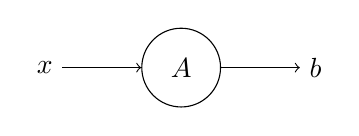
\begin{tikzpicture}[scale=0.8]
            \node[draw, circle, minimum size=1cm] (A) at (0,0) {$A$};
            \node[left=1cm of A] (x) {$x$};
            \node[right=1cm of A] (b) {$b$};
            \draw[->] (x) -- (A);
            \draw[->] (A) -- (b);
        \end{tikzpicture}

        \vspace{0.5cm}
        \footnotesize
        Example: Simulating MRI signal\\
        from a known image.

        \column{0.5\textwidth}
        \centering
        \textbf{Inverse Problems}
        \vspace{0.3cm}

        Given $b$, $A$ $\longrightarrow$ recover $x$

        \vspace{0.3cm}
        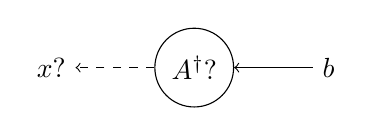
\begin{tikzpicture}[scale=0.8]
            \node[draw, circle, minimum size=1cm] (A) at (0,0) {$A^{\dagger}$?};
            \node[left=1cm of A] (x) {$x$?};
            \node[right=1cm of A] (b) {$b$};
            \draw[->, dashed] (A) -- (x);
            \draw[->] (b) -- (A);
        \end{tikzpicture}

        \vspace{0.5cm}
        \footnotesize
        Example: Reconstructing an image\\
        from MRI measurements.

    \end{columns}

    \vspace{0.3cm}
    \pause
    \begin{alertblock}{Inverse problems are harder}
        \begin{itemize}
            \item Often ill-conditioned (small noise $\to$ large errors)
            \item May be underdetermined (more unknowns than measurements)
            \item $A$ may not be square --- we need a pseudoinverse, not $A^{-1}$
            \item $A$ may be too large to store explicitly
        \end{itemize}
    \end{alertblock}
\end{frame}

% ===========================================================================
% SECTION 2: LINEAR SYSTEMS AS OPTIMIZATION
% ===========================================================================
\section{Linear Systems as Optimization}

\begin{frame}{From Linear Systems to Optimization}
    \textbf{Setup:} $A \in \R^{n \times n}$ symmetric positive definite (SPD), $b \in \R^n$.

    \vspace{0.3cm}
    Instead of solving $Ax = b$ directly, consider the \textbf{quadratic function}:
    \[
        f(x) = \frac{1}{2} x^T A x - b^T x
    \]

    \pause
    \vspace{0.3cm}
    \textbf{Why?} Because the gradient is:
    \[
        \nabla f(x) = A x - b = -(b - A x) = -r(x)
    \]
    where $r(x) = b - Ax$ is the \emph{residual}.

    \pause
    \vspace{0.3cm}
    \begin{block}{Equivalence}
        Setting $\nabla f(x^*) = 0$ gives $A x^* = b$.
        \\
        $\Rightarrow$ The unique minimizer of $f(x)$ is exactly the solution of $Ax = b$.
    \end{block}
\end{frame}

\begin{frame}{Geometric Intuition}
    \centering
    In 2D, $f(x) = \frac{1}{2}x^T A x - b^T x$ is a \textbf{paraboloid} (bowl).

    \vspace{0.2cm}
    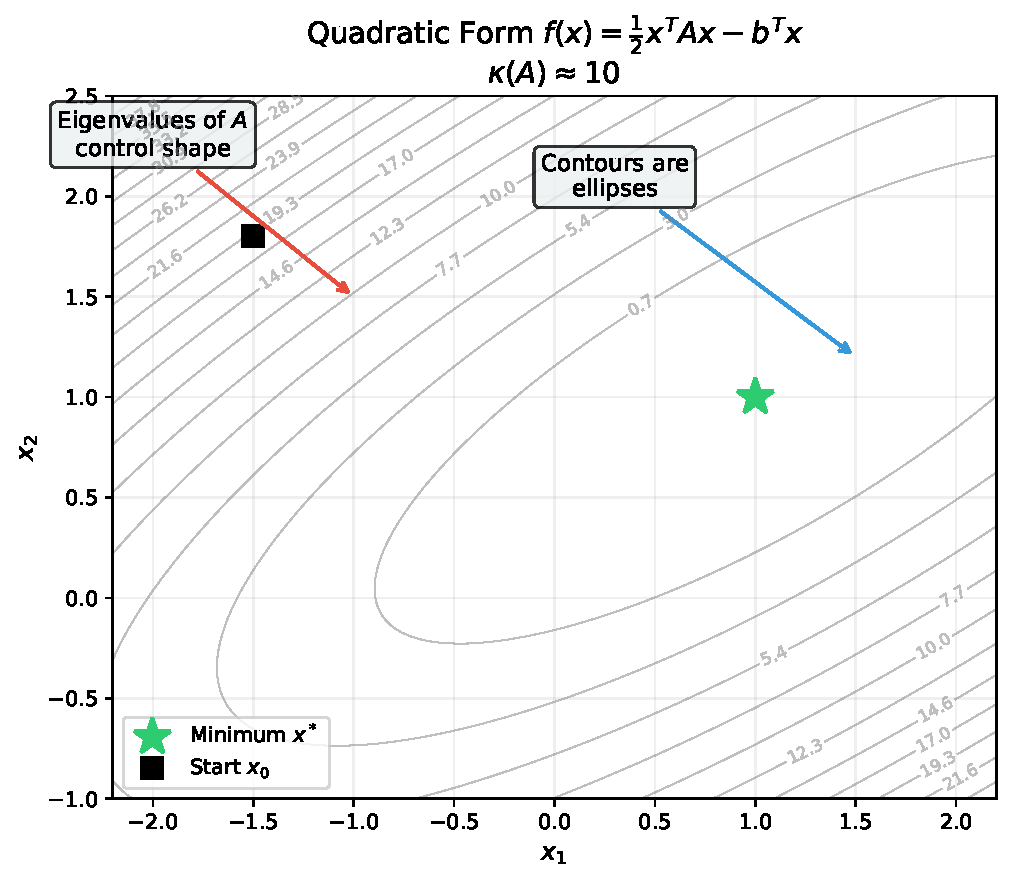
\includegraphics[width=0.52\textwidth]{figures/paraboloid_contours.pdf}

    \vspace{0.2cm}
    \begin{itemize}
        \item The level sets (contours of constant $f$) are \textbf{ellipses}
              whose shape is determined by the eigenvalues of $A$
        \item The condition number $\kappa(A) = \lambda_{\max}/\lambda_{\min}$ controls
              how ``stretched'' they are
        \item Minimizing $f(x)$ $\Leftrightarrow$ finding the bottom of the bowl
        \item Our goal: design an algorithm that walks to the minimum efficiently
    \end{itemize}
\end{frame}

\begin{frame}{Least Squares and the Normal Equations}
% NOTE: This frame appears early to connect optimization to linear systems,
% but also foreshadows the SENSE MRI formulation in Section 6.
    \textbf{The overdetermined case:} $A \in \R^{m \times n}$, $m > n$

    \[
        \min_x \; \|A x - b\|_2^2
    \]

    \pause
    \vspace{0.10cm}
    Expand the squared norm step by step:
    \begin{align*}
        \|A x - b\|_2^2 &= (Ax - b)^T (Ax - b) \\
        \onslide<3->{&= x^T A^T A x - (Ax)^T b - b^T (Ax) + b^T b \\}
        \onslide<4->{&= x^T A^T A x - 2 b^T A x + b^T b}
    \end{align*}

    \onslide<5->{
    \vspace{0.10cm}
    Take the gradient and set to zero $\Rightarrow$ \textbf{normal equations}:
    \[
        A^T A \, x = A^T b
    \]
    }

    \onslide<6->{
    \vspace{0.10cm}
    \begin{block}{Key property}
        $A^T A$ is always symmetric positive \emph{semidefinite}.
        If $A$ has full column rank, $A^T A$ is SPD --- we can use CG!
    \end{block}
    }

    \onslide<7->{
    \vspace{0.10cm}
    Later, we will use exactly this structure to formulate the \textbf{multi-coil MRI}
    reconstruction as a least-squares problem and solve it efficiently with CG.
    }
\end{frame}

% ===========================================================================
% SECTION 3: STEEPEST DESCENT
% ===========================================================================
\section{Steepest Descent}

\begin{frame}{Steepest Descent: The Natural First Attempt}
    \textbf{Idea:} At each step, move in the direction where $f$ decreases fastest.

    \vspace{0.2cm}
    {\footnotesize
    \begin{algorithm}[H]
        \caption{Steepest Descent for $Ax = b$}
        \begin{algorithmic}[1]
            \State Choose initial guess $x_0$
            \For{$k = 0, 1, 2, \ldots$}
                \State $r_k = b - A x_k$ \Comment{negative gradient}
                \State $\alpha_k = \dfrac{r_k^T r_k}{r_k^T A r_k}$
                       \Comment{exact line search}
                \State $x_{k+1} = x_k + \alpha_k r_k$
            \EndFor
        \end{algorithmic}
    \end{algorithm}
    }

    \pause
    \vspace{0.15cm}
    \begin{itemize}
        \item \textbf{Line search:} $\alpha_k$ minimizes $f(x_k + \alpha r_k)$ exactly
        \item Each step is orthogonal to the \emph{previous} step: $r_{k+1}^T r_k = 0$
        \item Simple, intuitive, \ldots but often painfully slow
    \end{itemize}
\end{frame}

\begin{frame}{Why Steepest Descent is Slow}
    \centering
    % NOTE: We show ONLY the SD trajectory here. CG is not introduced until
    % Section 4, so showing the CG path now would confuse students with an
    % unexplained blue trajectory. The full SD+CG comparison figure
    % (steepest_descent_vs_cg.pdf) is used later, after CG is introduced.
    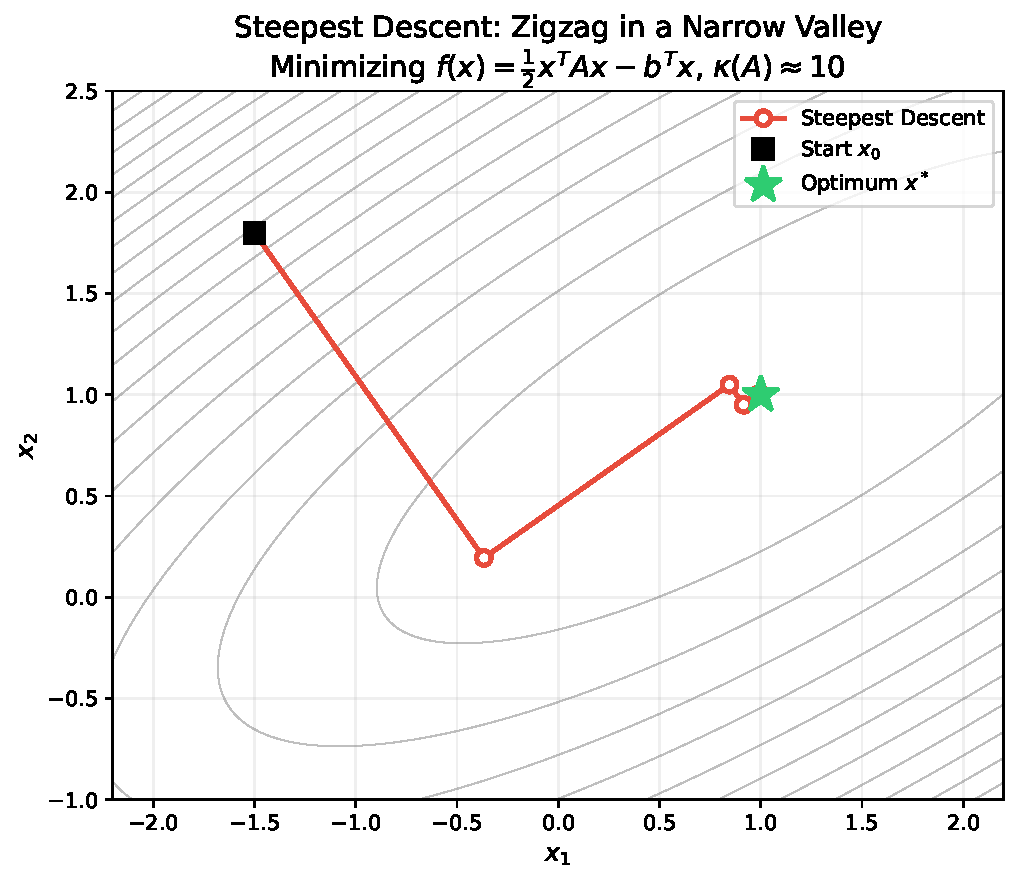
\includegraphics[width=0.52\textwidth]{figures/sd_zigzag_only.pdf}

    \vspace{0.15cm}
    \begin{itemize}
        \item Steepest descent \textbf{zigzags} along the narrow valley
        \item Each step undoes some progress of the previous step
        \item The convergence rate depends on $\kappa(A) = \lambda_{\max} / \lambda_{\min}$
    \end{itemize}

    \pause
    \vspace{0.15cm}
    Recall the \textbf{$A$-norm} (energy norm): $\|v\|_A = \sqrt{v^T A v}$.
    \\
    This measures ``error weighted by the system matrix'' --- directions
    corresponding to large eigenvalues are penalized more.

    \vspace{0.10cm}
    \begin{block}{Error bound for steepest descent (in $A$-norm)}
        \[
            \frac{\|x_k - x^*\|_A}{\|x_0 - x^*\|_A}
            \leq \left( \frac{\kappa - 1}{\kappa + 1} \right)^k
        \]
        When $\kappa \gg 1$, this approaches $1^k = 1$ --- essentially no progress!
    \end{block}
\end{frame}

\begin{frame}{Convergence Speed: SD vs CG}
    \centering
    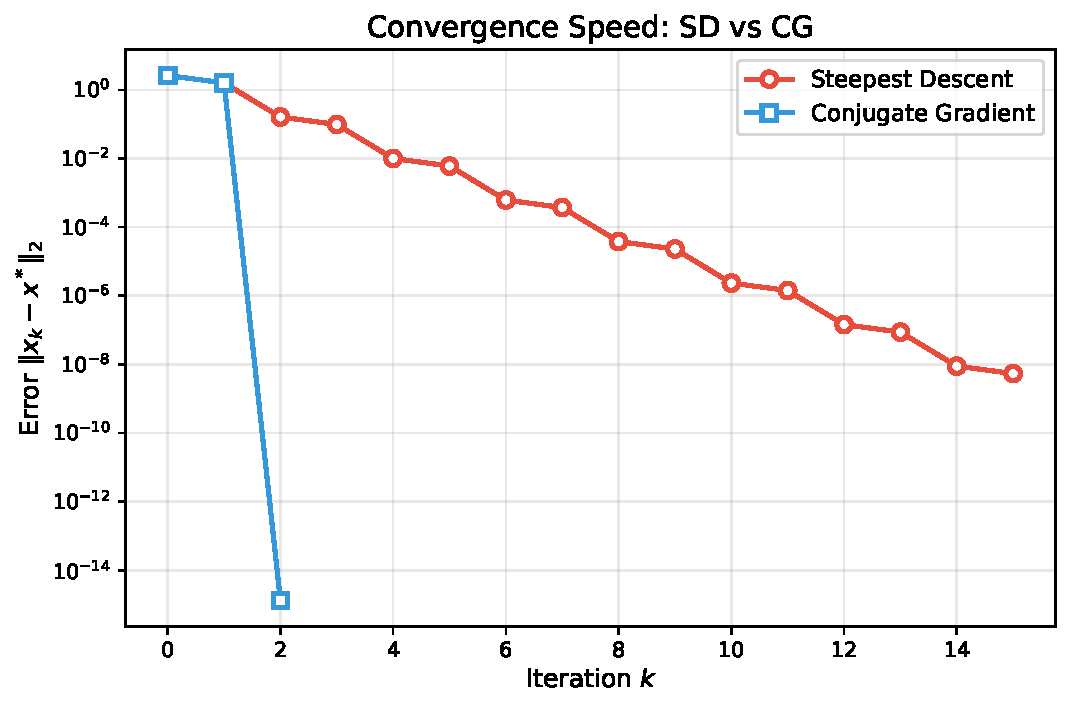
\includegraphics[width=0.50\textwidth]{figures/sd_vs_cg_error.pdf}

    \vspace{0.2cm}
    \textbf{The fundamental issue:} Steepest descent uses the \emph{gradient} as
    search direction, but gradient directions are not independent --- they
    interfere with each other.

    \pause
    \vspace{0.2cm}
    \begin{block}{What if we chose search directions that \emph{don't} interfere?}
        This is exactly the idea behind the \textbf{Conjugate Gradient} method.
    \end{block}
\end{frame}

% ===========================================================================
% SECTION 4: CONJUGATE GRADIENT
% ===========================================================================
\section{Conjugate Gradient}

\begin{frame}{A-Orthogonal (Conjugate) Directions}
    \textbf{Definition:} Two vectors $u, v \neq 0$ are \textbf{$A$-orthogonal}
    (or \emph{conjugate}) if:
    \[
        u^T A v = 0
    \]

    \vspace{0.2cm}
    \textbf{Geometric meaning:} Under the $A$-inner product $\langle u, v \rangle_A = u^T A v$,
    conjugate directions are orthogonal.

    \pause
    \vspace{0.2cm}
    \textbf{Why this matters:}
    \begin{itemize}
        \item If we have $n$ mutually $A$-orthogonal directions $\{p_0, \ldots, p_{n-1}\}$,
              we can reach $x^*$ in \emph{exactly $n$ steps}
        \item Each step along $p_k$ eliminates the error component in that direction
        \item Future steps don't reintroduce error in previous directions --- no zigzag!
    \end{itemize}

    \pause
    \vspace{0.2cm}
    \textbf{But how do we find these directions efficiently?}\\
    We don't want to compute all $n$ directions upfront ($O(n^3)$) --- that defeats the purpose!
\end{frame}

\begin{frame}{Building Conjugate Directions on the Fly}
    \textbf{CG's key idea:} Generate conjugate directions sequentially,
    one per iteration, using only the current residual.

    \vspace{0.2cm}
    \textbf{The recurrence:}
    \begin{align*}
        p_0 &= r_0 = b - A x_0 \\[0.2cm]
        p_{k+1} &= r_{k+1} + \beta_k p_k
    \end{align*}

    \vspace{0.15cm}
    where $\beta_k = \dfrac{r_{k+1}^T r_{k+1}}{r_k^T r_k}$ ensures $p_{k+1}^T A p_k = 0$.

    \pause
    \vspace{0.2cm}
    \textbf{Properties of CG (what makes it beautiful):}
    \begin{enumerate}
        \item The residuals $r_0, r_1, \ldots$ are mutually orthogonal: $r_i^T r_j = 0$ for $i \neq j$
        \item The search directions are mutually $A$-orthogonal: $p_i^T A p_j = 0$ for $i \neq j$
        \item $x_k$ minimizes $f(x)$ over the \emph{Krylov subspace}
              $\mathcal{K}_k = \operatorname{span}\{b, Ab, \ldots, A^{k-1}b\}$
        \item Only one matrix-vector product $A p_k$ per iteration
    \end{enumerate}
\end{frame}

\begin{frame}{CG Algorithm}
    {\scriptsize
    \begin{algorithm}[H]
        \caption{Conjugate Gradient (Hestenes \& Stiefel, 1952)}
        \begin{algorithmic}[1]
            \State $x_0 = 0$ (or any initial guess)
            \State $r_0 = b - A x_0$
            \State $p_0 = r_0$
            \For{$k = 0, 1, 2, \ldots$ until convergence}
                \State $\alpha_k = \dfrac{r_k^T r_k}{p_k^T A p_k}$
                      \Comment{step size}
                \State $x_{k+1} = x_k + \alpha_k p_k$
                      \Comment{update solution}
                \State $r_{k+1} = r_k - \alpha_k A p_k$
                      \Comment{update residual}
                \State $\beta_k = \dfrac{r_{k+1}^T r_{k+1}}{r_k^T r_k}$
                      \Comment{conjugacy coeff.}
                \State $p_{k+1} = r_{k+1} + \beta_k p_k$
                      \Comment{new direction}
            \EndFor
        \end{algorithmic}
    \end{algorithm}
    }

    \vspace{0.10cm}
    \begin{itemize}
        \item \textbf{Cost per iteration:} one $A p_k$, two inner products, three vector updates
        \item \textbf{Memory:} only need $x, r, p, Ap$ --- four vectors
        \item \textbf{For sparse $A$:} $O(\text{nnz})$ per iteration vs $O(n^3)$ for direct solver
    \end{itemize}
\end{frame}

\begin{frame}{Why CG Works: Krylov Subspace Interpretation}
    \textbf{Krylov subspace of order $k$:}
    \[
        \mathcal{K}_k(A, b) = \operatorname{span}\{b, Ab, A^2 b, \ldots, A^{k-1} b\}
    \]

    \vspace{0.15cm}
    \textbf{CG chooses $x_k$ to be the \emph{optimal} solution within $\mathcal{K}_k$:}
    \[
        x_k = \arg\min_{x \in x_0 + \mathcal{K}_k} \|x - x^*\|_A
    \]
    where $\|v\|_A = \sqrt{v^T A v}$ is the \emph{$A$-norm} (energy norm).

    \pause
    \vspace{0.2cm}
    \textbf{Three equivalent views of CG (they all describe the same thing):}
    \begin{enumerate}
        \item An algorithm that generates $A$-orthogonal search directions
        \item An algorithm that minimizes $\|x_k - x^*\|_A$ over $\mathcal{K}_k$
        \item An algorithm that orthogonalizes the residuals via Lanczos
    \end{enumerate}

    \vspace{0.15cm}
    \begin{block}{Finite termination}
        In exact arithmetic, CG finds $x^*$ in at most $n$ iterations.
        In practice, we stop much earlier --- the approximation is already excellent.
    \end{block}
\end{frame}

% ===========================================================================
% SECTION 5: CONVERGENCE
% ===========================================================================
\section{Convergence Properties}

\begin{frame}{Convergence Rate: The Condition Number Story}
    \textbf{Steepest Descent (in $A$-norm):}
    \[
        \frac{\|x_k - x^*\|_A}{\|x_0 - x^*\|_A}
        \leq \left( \frac{\kappa - 1}{\kappa + 1} \right)^k
    \]

    \textbf{Conjugate Gradient (in $A$-norm):}
    \[
        \frac{\|x_k - x^*\|_A}{\|x_0 - x^*\|_A}
        \leq 2 \left( \frac{\sqrt{\kappa} - 1}{\sqrt{\kappa} + 1} \right)^k
    \]
    where $\kappa = \kappa(A) = \lambda_{\max} / \lambda_{\min}$.

    \pause
    \vspace{0.2cm}
    \begin{alertblock}{CG replaces $\kappa$ with $\sqrt{\kappa}$ --- a dramatic improvement!}
        \begin{tabular}{c|c|c}
            $\kappa$ & SD factor/iter & CG factor/iter \\
            \hline
            1        & 0.000 (instant) & 0.000 (instant) \\
            10       & 0.818 & 0.520 \\
            100      & 0.980 & 0.819 \\
            1000     & 0.998 & 0.939 \\
        \end{tabular}
    \end{alertblock}

    \pause
    \vspace{0.2cm}
    \begin{block}{Practical consequence: Preconditioning}
        Replace $Ax = b$ with $M^{-1}Ax = M^{-1}b$,
        where $M \approx A$ but $M^{-1}$ is easy to apply.
        $\Rightarrow$ Improve $\kappa \to$ faster convergence.
    \end{block}
\end{frame}

\begin{frame}{Beyond the Condition Number: Eigenvalue Clustering}
    The bound in terms of $\kappa$ is a \emph{worst-case} bound.
    Real convergence depends on the \textbf{distribution} of eigenvalues.
    \textbf{CG typically converges much faster than the bound predicts!}

    \vspace{0.15cm}
    \centering
    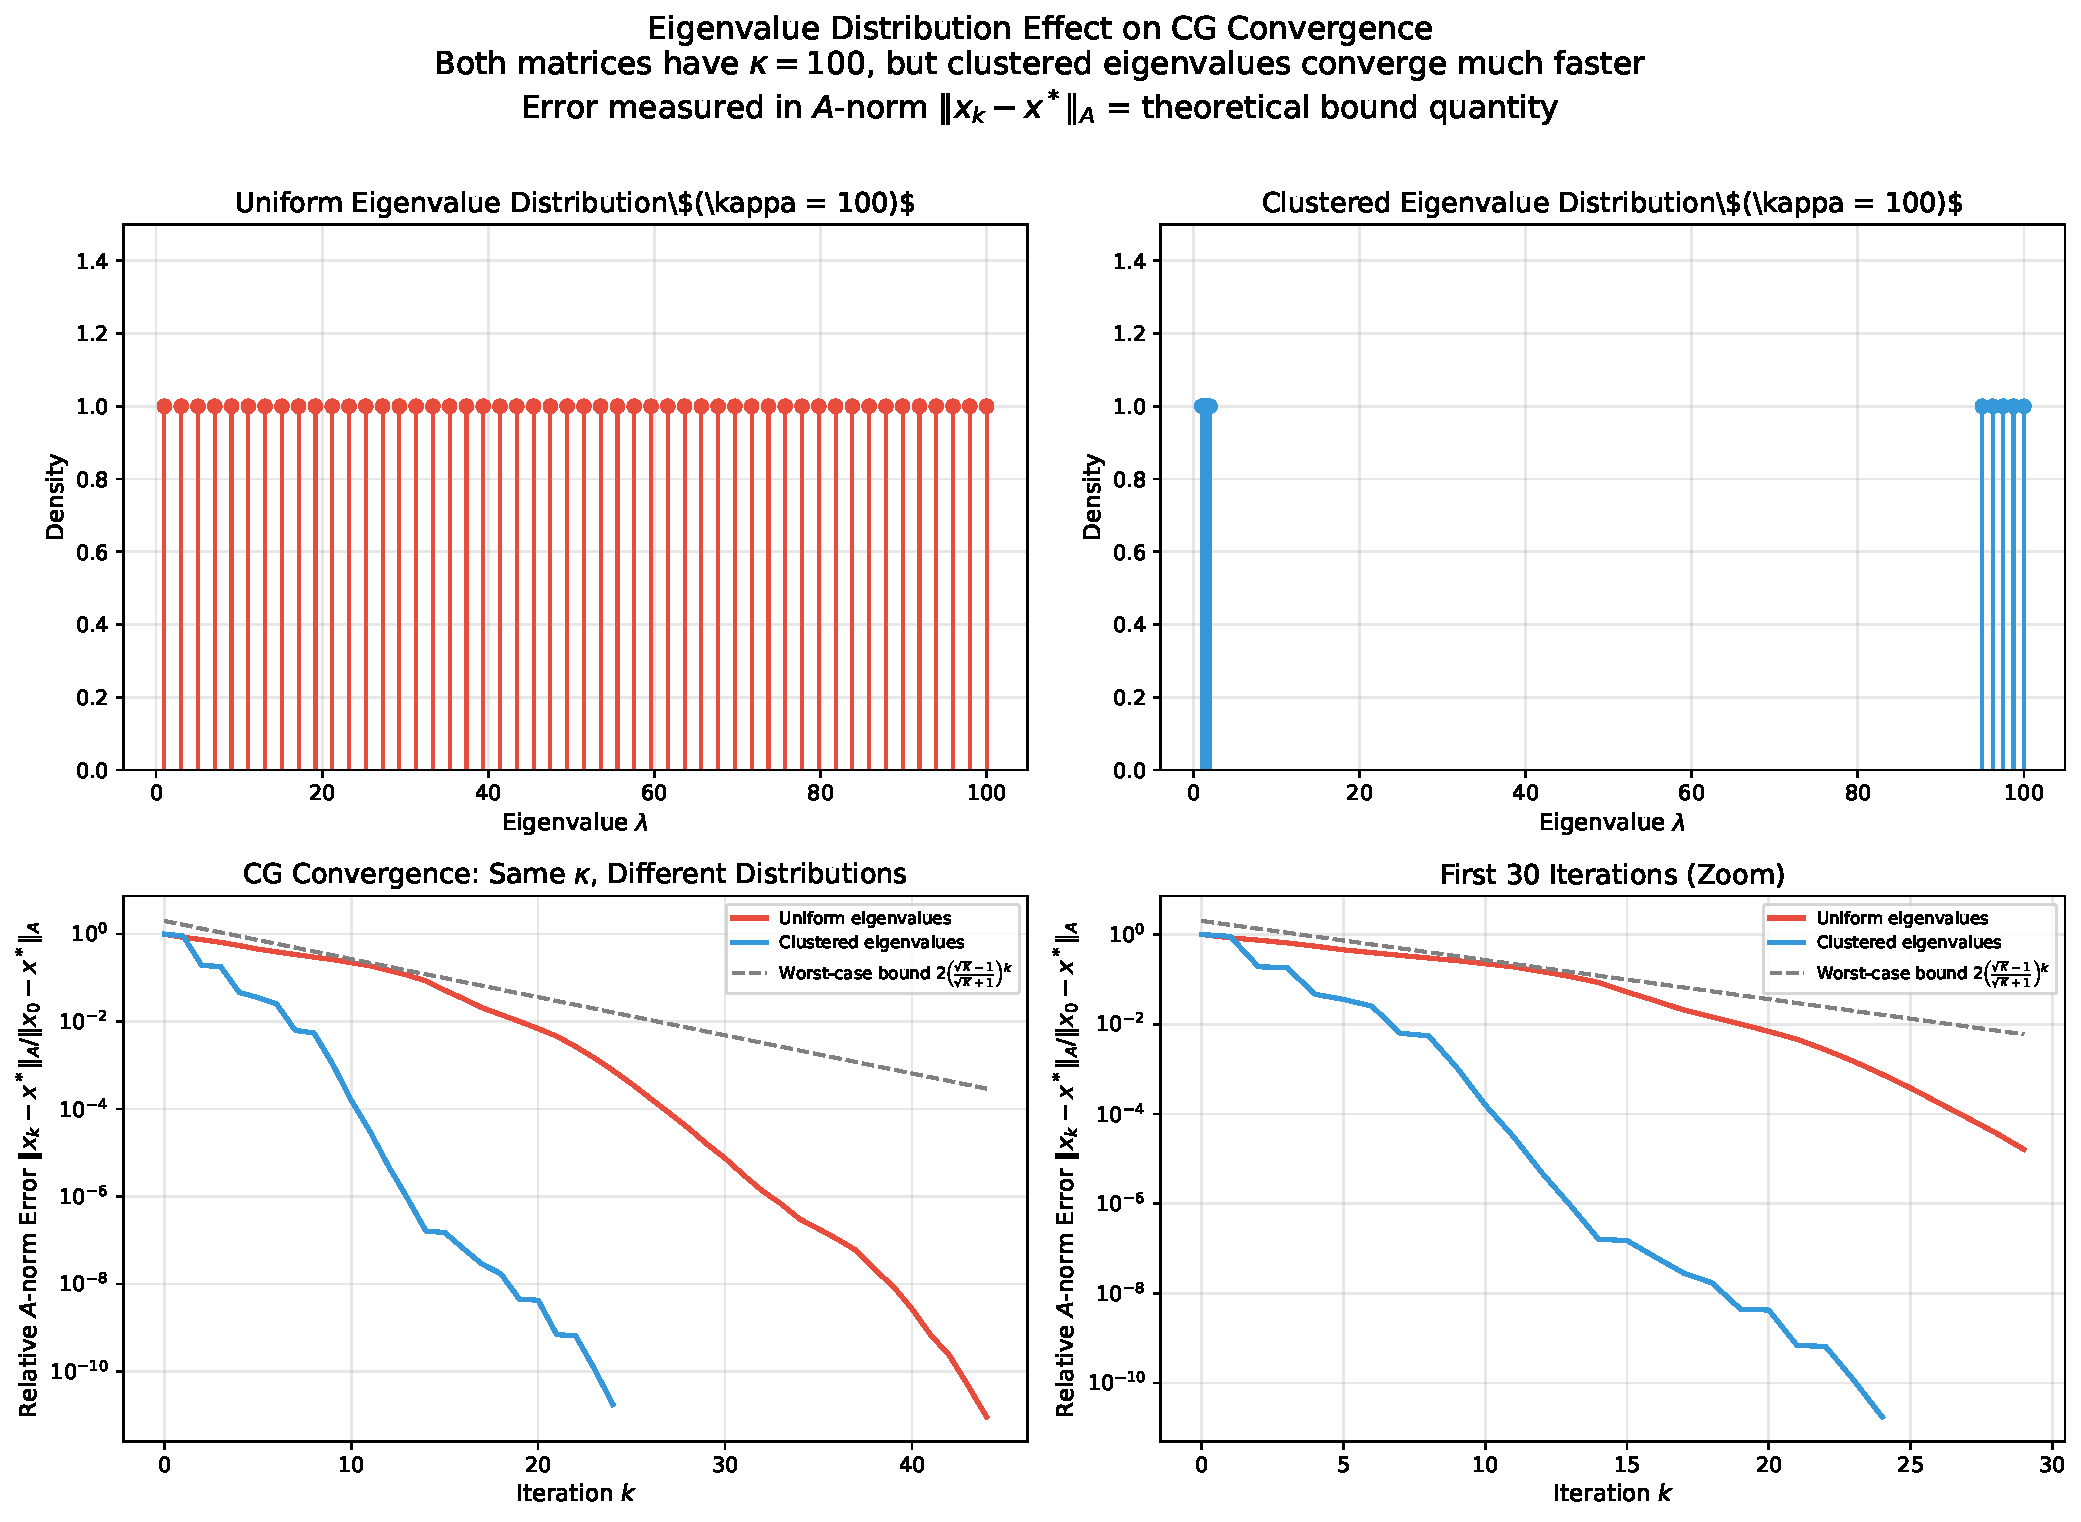
\includegraphics[width=0.72\textwidth]{figures/eigenvalue_illustration.pdf}

    \vspace{0.15cm}
    \begin{itemize}
        \item \textbf{Left:} Uniform eigenvalues in $[1, 100]$ --- slow convergence
        \item \textbf{Right:} $n-5$ eigenvalues in $[1, 2]$, 5 in $[95, 100]$ --- fast convergence
        \item Both have $\kappa = 100$, but the clustered case converges \textbf{much} faster
        \item The worst-case bound is identical for both matrices --- it cannot distinguish them!
    \end{itemize}

    \pause
    \textbf{Rule of thumb:} CG effectively ``eliminates'' each cluster of eigenvalues
    in roughly one iteration per cluster.
\end{frame}

\begin{frame}{Practical CG: Stopping Criteria and Preconditioning}
    \textbf{When to stop?}
    \begin{itemize}
        \item Monitor $\|r_k\|_2 / \|b\|_2$ (relative residual)
        \item Stop when below a tolerance (e.g., $10^{-6}$ for well-conditioned systems)
        \item In inverse problems: stop before fitting the noise!
              (This is the \emph{semiconvergence} phenomenon --- the error
              to the true solution may increase after some point, even though
              the residual keeps decreasing)
    \end{itemize}

    \pause
    \vspace{0.2cm}
    \textbf{Preconditioning strategies for CG:}
    \begin{itemize}
        \item \textbf{Jacobi (diagonal):} $M = \operatorname{diag}(A)$ --- simple, sometimes effective
        \item \textbf{Incomplete Cholesky:} Approximate factorization with limited fill
        \item \textbf{Multigrid:} Excellent for elliptic PDEs, $O(n)$ complexity
        \item \textbf{For MRI specifically:} Density compensation, circulant preconditioners
    \end{itemize}
\end{frame}

% ===========================================================================
% SECTION 6: MULTI-COIL MRI RECONSTRUCTION
% ===========================================================================
\section{Multi-Coil MRI Reconstruction}

\begin{frame}{MRI in One Slide}
    \textbf{Magnetic Resonance Imaging} measures the signal from excited protons
    in a strong magnetic field.

    \vspace{0.15cm}
    \begin{columns}[T]
        \column{0.55\textwidth}
        \begin{itemize}
            \item Protons precess at the Larmor frequency $\omega = \gamma B_0$
            \item \textbf{Gradient fields} $G_x, G_y, G_z$ encode spatial position
                  into frequency and phase
            \item The measured signal in \textbf{k-space} is the 2D Fourier transform
                  of the proton density (image):
                  \[
                      s(k_x, k_y) = \iint \rho(x, y)\, e^{-j2\pi(k_x x + k_y y)} \,dx\,dy
                  \]
            \item \textbf{k-space} $=$ spatial frequency domain of the image
        \end{itemize}

        \column{0.45\textwidth}
        \centering
        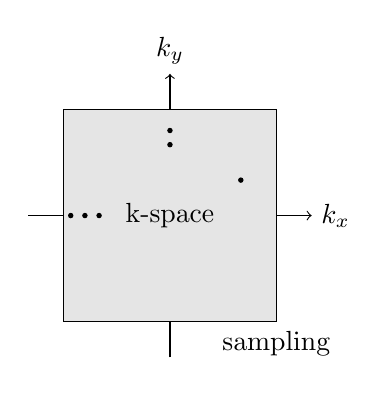
\begin{tikzpicture}[scale=0.9]
            \draw[->] (-2,0) -- (2,0) node[right] {$k_x$};
            \draw[->] (0,-2) -- (0,2) node[above] {$k_y$};
            \draw[fill=gray!20] (-1.5,-1.5) rectangle (1.5,1.5);
            \node at (0,0) {k-space};
            \node at (1.5,-1.8) {sampling};
            \draw[fill=black] (-1.4,0) circle (0.03);
            \draw[fill=black] (-1.2,0) circle (0.03);
            \draw[fill=black] (-1.0,0) circle (0.03);
            \draw[fill=black] (0,1.2) circle (0.03);
            \draw[fill=black] (0,1.0) circle (0.03);
            \draw[fill=black] (1.0,0.5) circle (0.03);
        \end{tikzpicture}
    \end{columns}

    \vspace{0.15cm}
    \pause
    \begin{alertblock}{The speed problem}
        To form an image, we must sample k-space line by line.
        A full scan takes minutes --- patients move, creating artifacts.
        \textbf{Can we sample fewer lines and still reconstruct the image?}
    \end{alertblock}
\end{frame}

\begin{frame}{Multi-Coil Acquisition: The Key to Acceleration}
    Modern MRI scanners use \textbf{arrays of receiver coils} placed around the patient.

    \vspace{0.15cm}
    \centering
    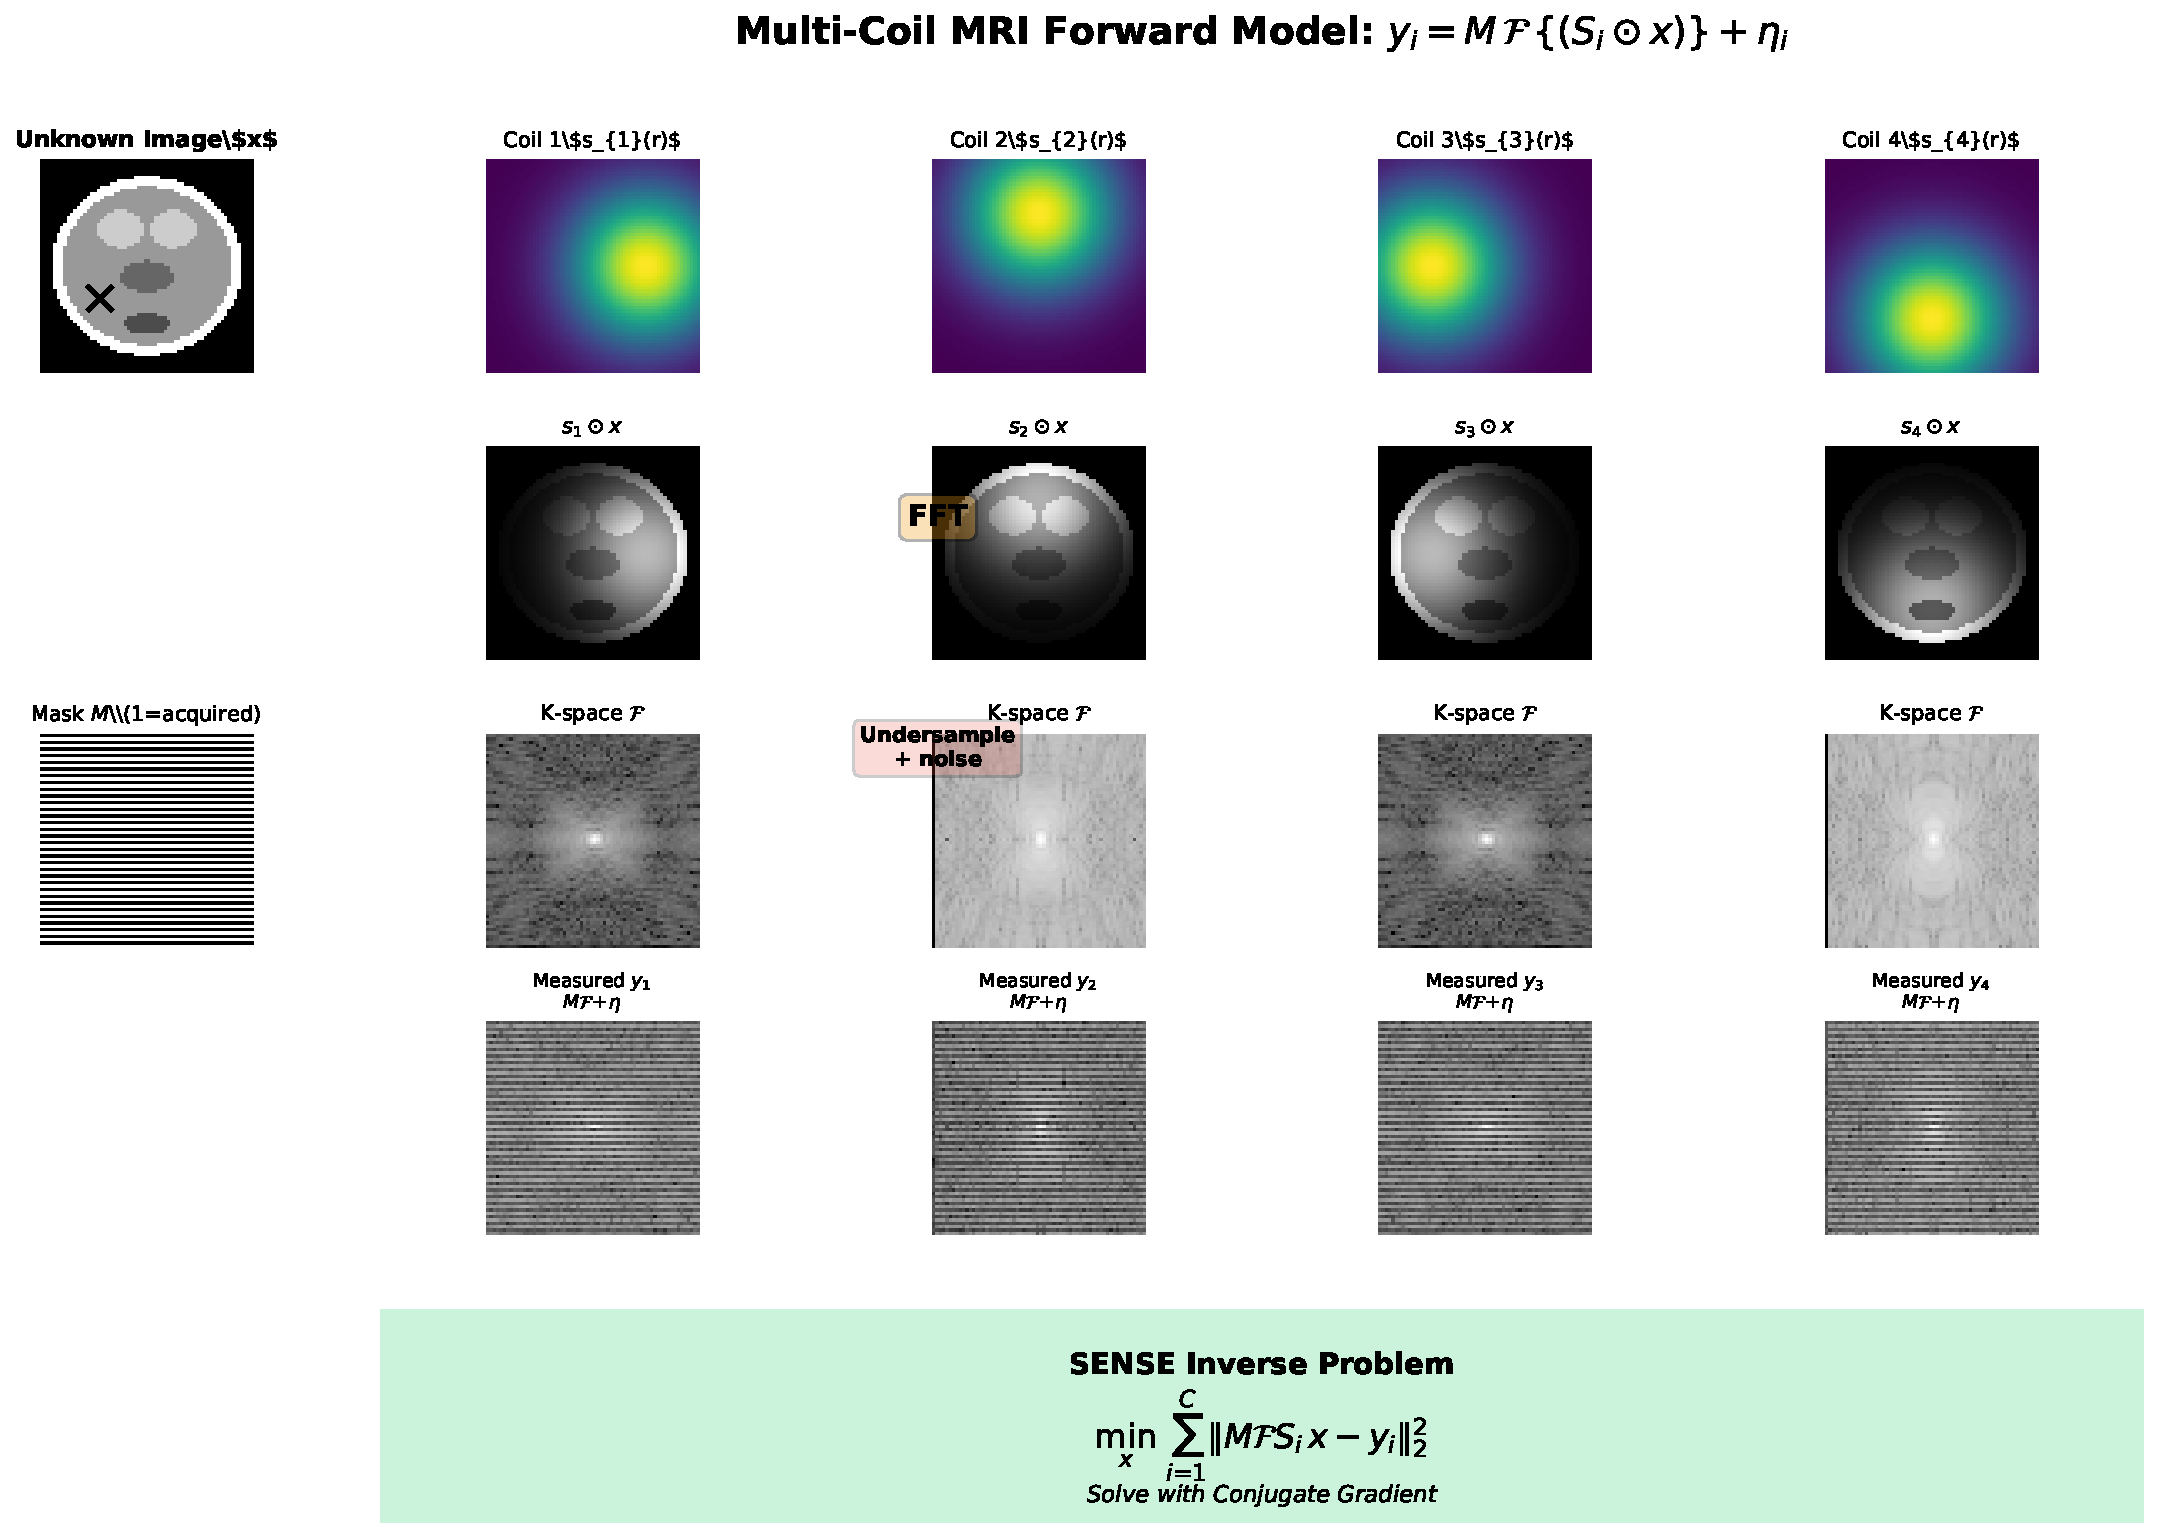
\includegraphics[width=0.52\textwidth]{figures/mri_acquisition_model.pdf}

    \vspace{0.15cm}
    \begin{columns}[T]
        \column{0.65\textwidth}
        \begin{itemize}
            \item Each coil $i$ has a \textbf{sensitivity profile} $s_i(\mathbf{r})$ ---
                  it sees the object differently depending on position
            \item Coil sensitivities provide \emph{spatial encoding} that can replace
                  some gradient encoding steps
            \item This allows us to \textbf{undersample} k-space (skip lines)
                  and still recover the image $\to$ faster scans!
        \end{itemize}

        \column{0.35\textwidth}
        \centering
        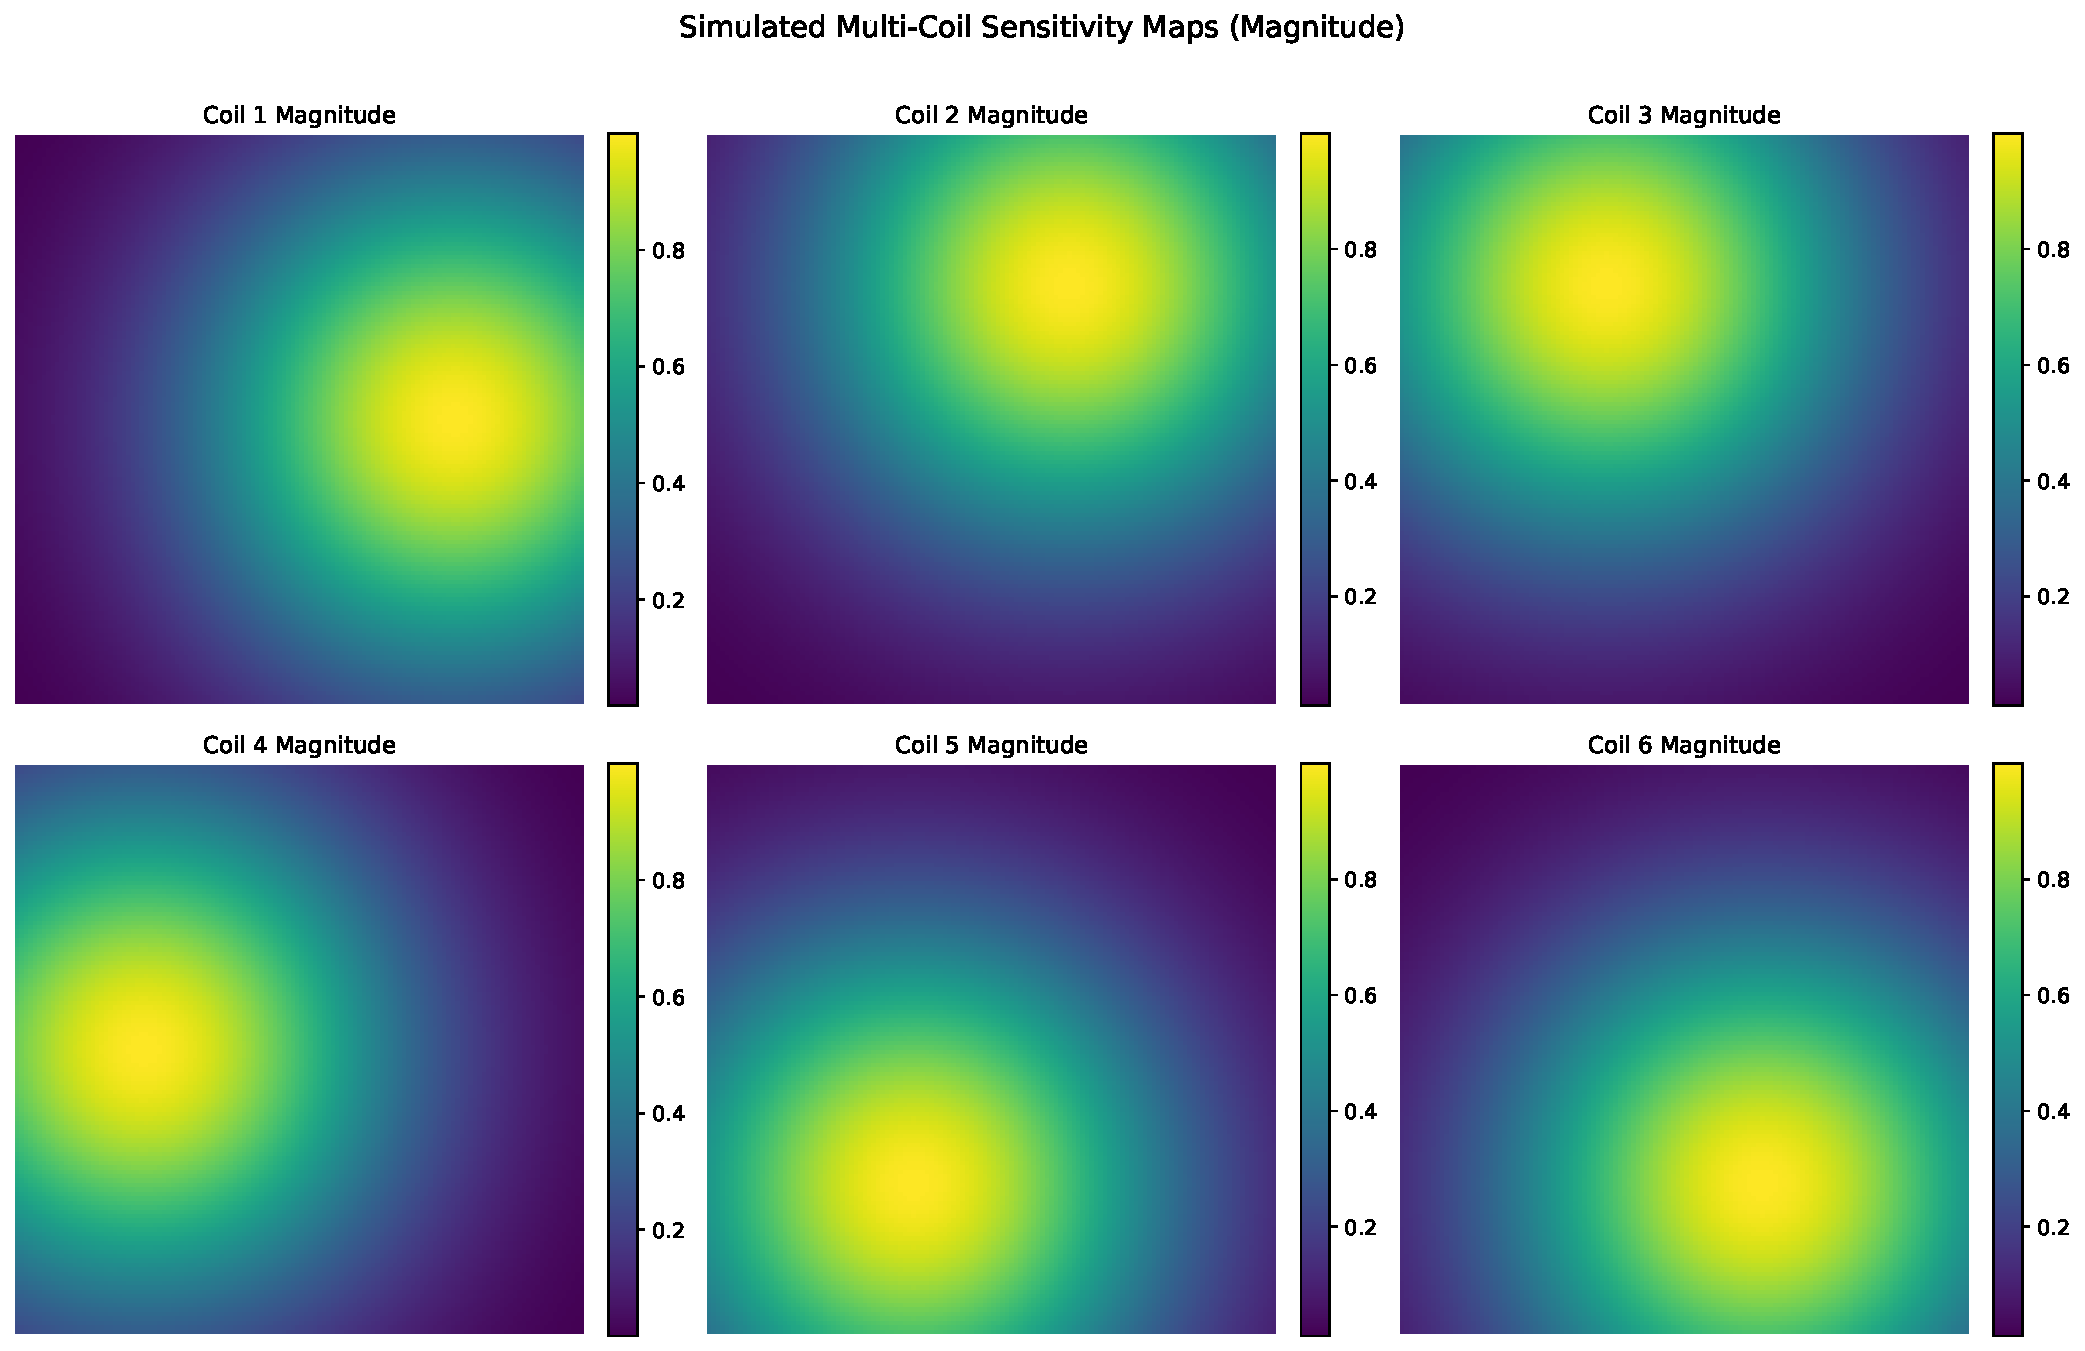
\includegraphics[width=\textwidth]{figures/coil_sensitivity_maps.pdf}

        \vspace{0.1cm}
        {\footnotesize Example coil sensitivity\\
        magnitudes (6 coils)}
    \end{columns}
\end{frame}

\begin{frame}{The SENSE Model (Pruessmann et al., 1999)}
    For $C$ coils with sensitivities $\{s_i(\mathbf{r})\}_{i=1}^C$, the forward model:
    \[
        y_i = M \mathcal{F} \{ s_i \odot x \} + \eta_i, \qquad i = 1, \ldots, C
    \]

    \vspace{0.15cm}
    \begin{itemize}
        \item $x \in \C^N$: unknown image (flattened)
        \item $s_i \in \C^N$: coil sensitivity map (diagonal operator $S_i$)
        \item $\mathcal{F}$: 2D discrete Fourier transform (unitary)
        \item $M$: Cartesian undersampling mask (keeps every $R$-th line)
        \item $y_i$: measured k-space data from coil $i$
        \item $\eta_i$: complex Gaussian noise
    \end{itemize}

    \pause
    \vspace{0.2cm}
    \textbf{The SENSE inverse problem (least squares):}
    \[
        \min_x \; \sum_{i=1}^{C} \big\| M \mathcal{F} S_i x - y_i \big\|_2^2
    \]

    This has the form $\min_x \|A x - y\|_2^2$ --- we can apply \textbf{CG}!
\end{frame}

\begin{frame}{SENSE Normal Equations for CG}
    \textbf{Step 1: Form the normal equations}\\
    Expanding the least-squares cost and setting the gradient to zero:
    \[
        \underbrace{\left( \sum_{i=1}^{C} S_i^H \mathcal{F}^H M \mathcal{F} S_i \right)}_{A_{\text{norm}}}
        x \;=\;
        \underbrace{\sum_{i=1}^{C} S_i^H \mathcal{F}^H y_i}_{b}
    \]

    \vspace{0.15cm}
    \textbf{Step 2: Apply $A_{\text{norm}}$ implicitly via FFTs}\\
    For any vector $v$, compute $A_{\text{norm}} v$ without forming the matrix:
    \begin{enumerate}
        \item For each coil $i$: multiply by $s_i$, FFT, apply mask $M$, IFFT, multiply by $\overline{s_i}$
        \item Sum over all coils
    \end{enumerate}

    \vspace{0.15cm}
    \textbf{Step 3: Ensure positive definiteness}\\
    $A_{\text{norm}}$ is Hermitian positive \emph{semidefinite}. With aggressive
    undersampling, its nullspace may contain nonzero vectors, causing CG to break
    down. The fix: add a small \textbf{Tikhonov regularization} term:
    \[
        (A_{\text{norm}} + \lambda I) \, x = b, \qquad \lambda > 0
    \]
    This shifts all eigenvalues by $\lambda$, making the system strictly
    positive definite with only a small bias cost.

    \pause
    \vspace{0.15cm}
    \begin{block}{Why CG works here}
        The coil sensitivities provide the ``missing'' spatial information
        that was lost by skipping k-space lines. CG efficiently finds the image
        consistent with \emph{all} coil measurements simultaneously.
    \end{block}
\end{frame}

\begin{frame}{Reconstruction Results: Zero-Filled vs CG}
    \centering
    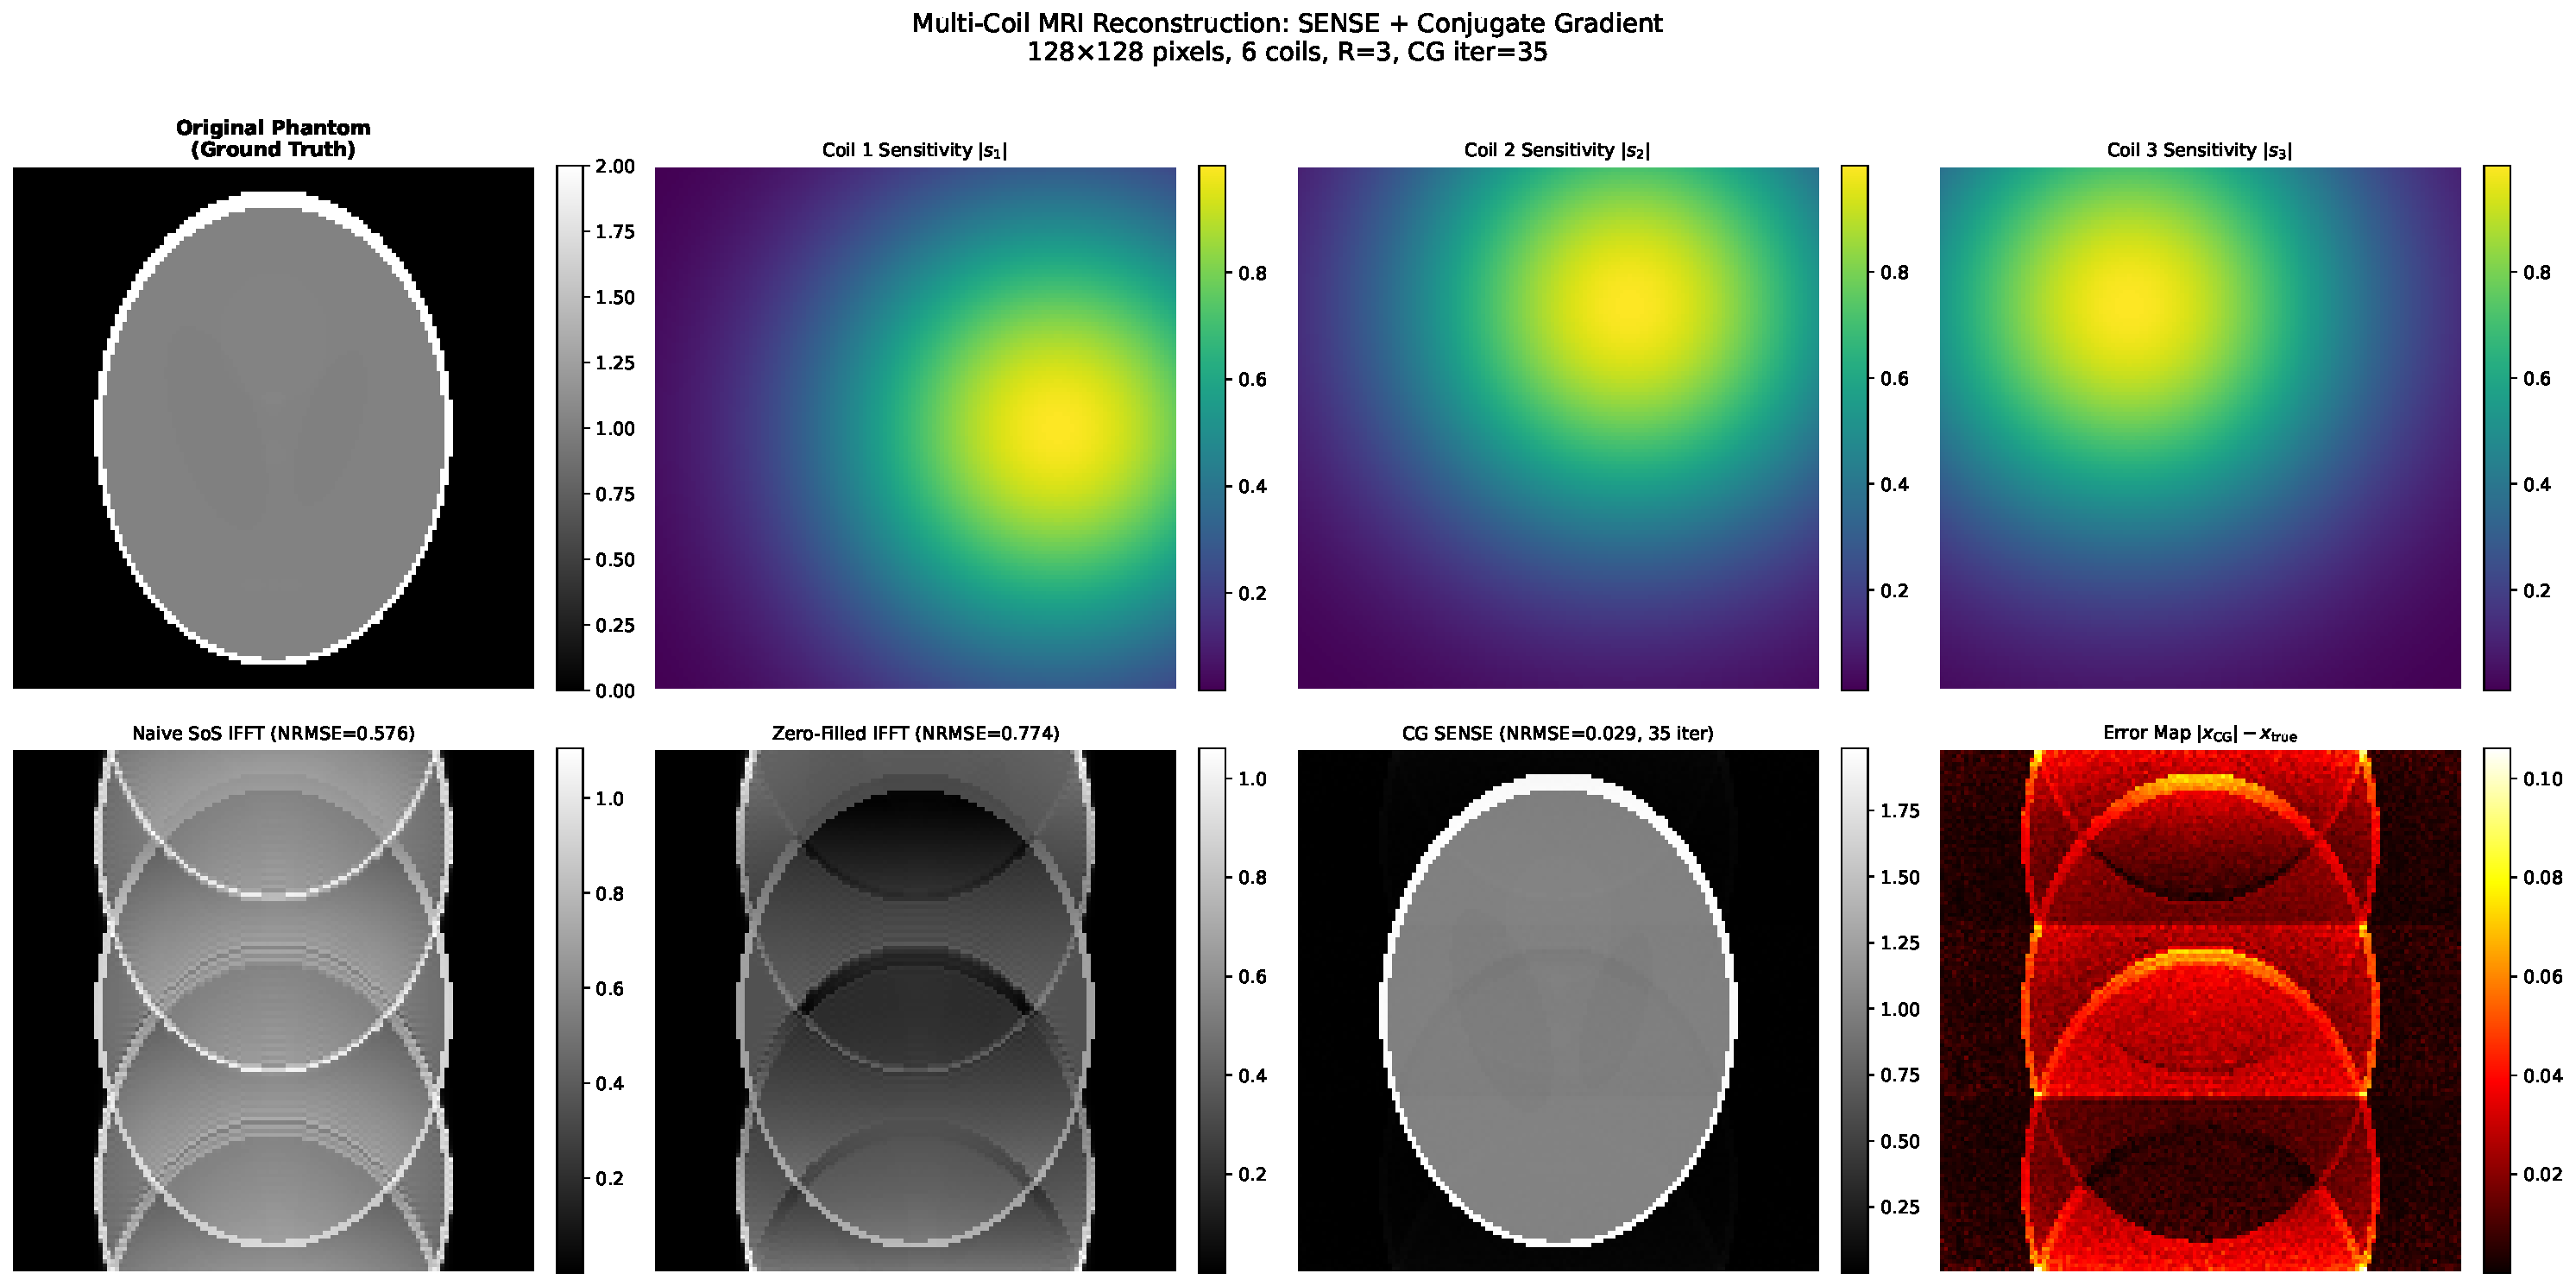
\includegraphics[width=0.78\textwidth]{figures/mri_reconstruction_results.pdf}

    \vspace{0.15cm}
    \begin{itemize}
        \item \textbf{Zero-filled IFFT:} Fast but shows severe aliasing artifacts
              (overlapping replicas from undersampling)
        \item \textbf{CG (SENSE):} Uses coil sensitivity information to separate
              the overlapping signals --- aliasing is removed
        \item CG converges in $\sim$10--20 iterations for typical acceleration factors
    \end{itemize}
\end{frame}

\begin{frame}{CG Convergence and Semiconvergence}
    \centering
    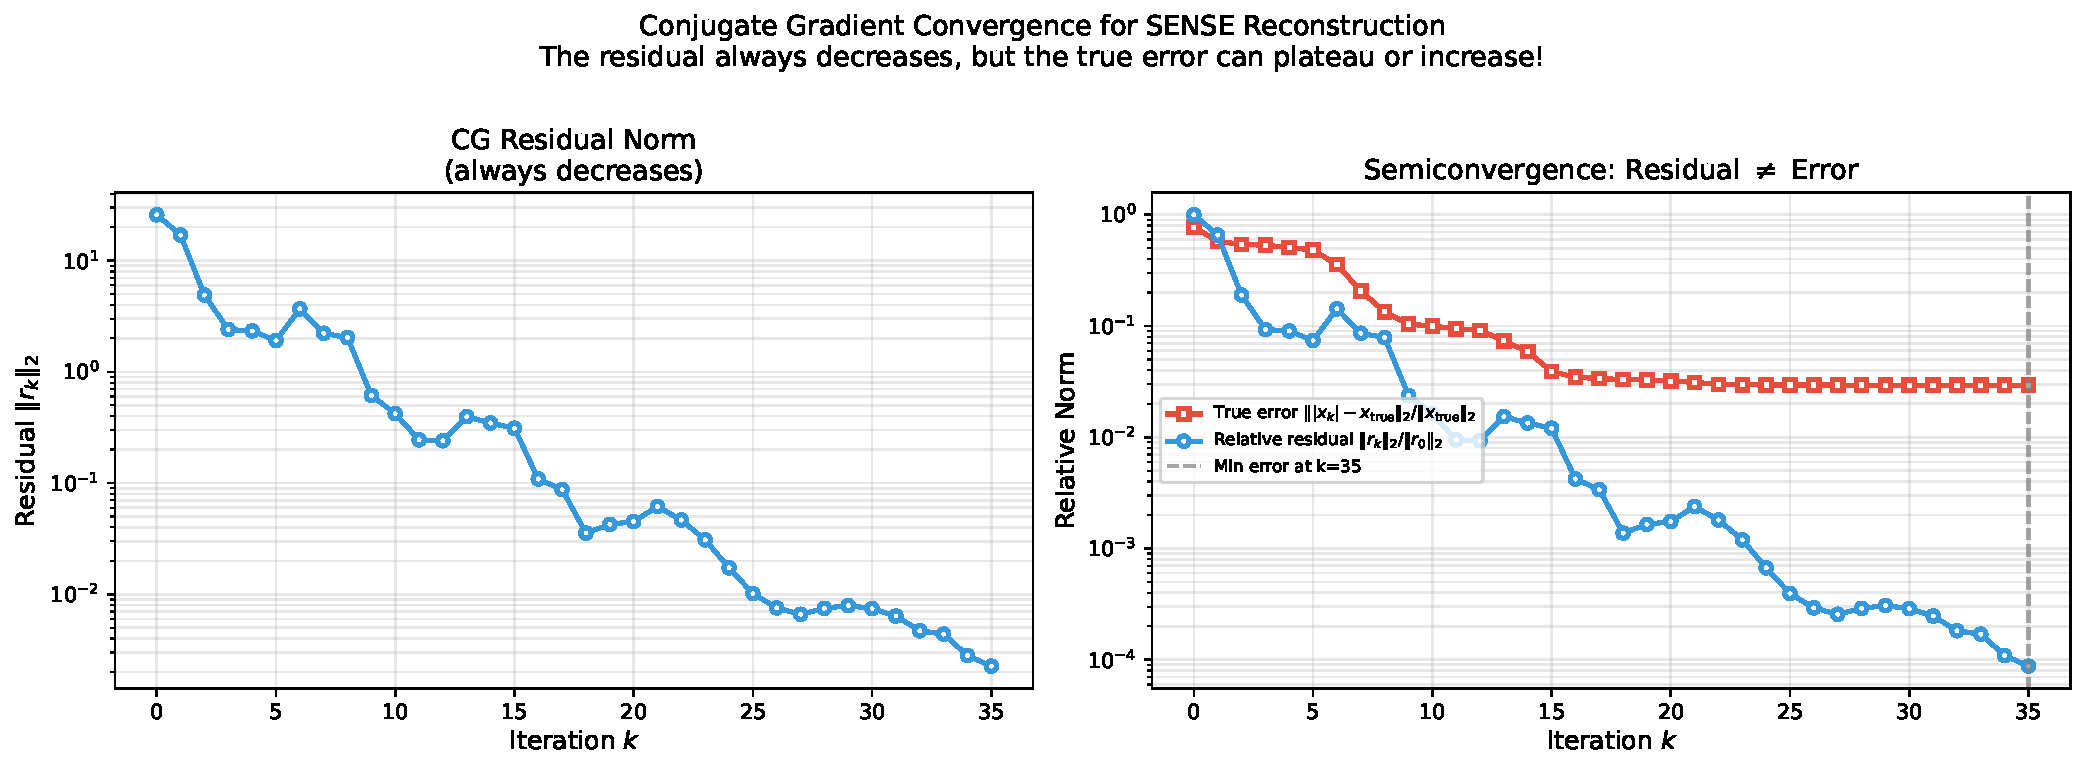
\includegraphics[width=0.72\textwidth]{figures/mri_cg_convergence.pdf}

    \vspace{0.2cm}
    \begin{itemize}
        \item Residual drops rapidly in the first few iterations
        \item After $\sim$15 iterations, we're close to the true image
        \item \textbf{Warning:} In inverse problems, the residual \emph{always} decreases
              monotonically, but the true reconstruction error can start to
              \emph{increase} as we begin to fit the noise --- this is \textbf{semiconvergence}
        \item The effective condition number depends on:
              \begin{itemize}
                  \item Coil geometry (well-separated coils $\to$ better conditioning)
                  \item Undersampling factor $R$ (higher $R$ $\to$ worse conditioning)
                  \item Regularization parameter $\lambda$
              \end{itemize}
    \end{itemize}
\end{frame}

% ===========================================================================
% SECTION 7: SUMMARY
% ===========================================================================
\section{Summary}

\begin{frame}{Summary: What We Learned}
    \begin{enumerate}
        \item \textbf{Iterative solvers} are essential for large-scale linear systems
              where direct methods are too expensive.

        \item \textbf{Steepest descent} is intuitive but suffers from zigzagging
              --- convergence depends on $\kappa(A)$, with rate $((\kappa-1)/(\kappa+1))^k$.

        \item \textbf{Conjugate Gradient} fixes this by using $A$-orthogonal
              search directions, replacing $\kappa$ with $\sqrt{\kappa}$ in the
              convergence bound, and converging in at most $n$ steps.

        \item \textbf{Convergence} depends on eigenvalue distribution, not just
              condition number --- clustered eigenvalues mean faster convergence.
              The condition number bound is a worst-case; real CG is often much faster.

        \item \textbf{Multi-coil MRI} uses arrays of receiver coils with distinct
              sensitivity profiles to enable undersampled acquisition.

        \item \textbf{SENSE reconstruction} formulates the problem as a linear
              least-squares system; CG solves it efficiently using implicit
              matrix-vector products via FFTs. Regularization ($+\lambda I$) ensures
              positive definiteness and controls noise amplification.
    \end{enumerate}

    \vspace{0.2cm}
    \begin{block}{CG is everywhere}
        CG is one of the most widely used algorithms in scientific computing ---
        from PDE solvers to optimization (nonlinear CG) to machine learning
        (CG for kernel methods, second-order optimization).
    \end{block}
\end{frame}

\begin{frame}{Further Reading and Code}
    \textbf{Classic papers:}
    \begin{itemize}
        \item Hestenes \& Stiefel (1952). ``Methods of Conjugate Gradients for Solving
              Linear Systems.'' \textit{J. Res. Natl. Bur. Stand.}
        \item Pruessmann et al. (1999). ``SENSE: Sensitivity Encoding for Fast MRI.''
              \textit{Magn. Reson. Med.}
    \end{itemize}

    \vspace{0.2cm}
    \textbf{Textbooks:}
    \begin{itemize}
        \item Trefethen \& Bau (1997). \textit{Numerical Linear Algebra}. SIAM.
        \item Nocedal \& Wright (2006). \textit{Numerical Optimization}. Springer.
        \item Shewchuk (1994). ``An Introduction to the Conjugate Gradient Method
              Without the Agonizing Pain.'' (free online --- highly recommended!)
    \end{itemize}

    \vspace{0.2cm}
    \textbf{Code for this lecture:}
    \begin{itemize}
        \item \texttt{code/illustrations/} --- Python scripts that generate the figures
        \item \texttt{code/mri\_demo/} --- Full SENSE+CG reconstruction demo
        \item All code is self-contained and runnable; experiment with different
              parameters to build intuition!
    \end{itemize}
\end{frame}

\begin{frame}
    \centering
    \Huge
    \textbf{Thank you!}

    \vspace{1cm}
    \Large
    Questions?

    \vspace{1.5cm}
    \normalsize
    \textit{``The CG method is the most important iterative method for solving
    large sparse systems of linear equations.''}
    \\
    --- Yousef Saad
\end{frame}

\end{document}
